\documentclass[border=3pt]{standalone}
% Preâmbulo compartilhado pelos diagramas TikZ da aula 8 de IHC (Design de IHC)
\usepackage[T1]{fontenc}
\usepackage[utf8]{inputenc}
\usepackage{lmodern}
\usepackage{amsmath}
\usepackage{xcolor}
\usepackage{tikz}
\usetikzlibrary{arrows.meta,angles,quotes,decorations.pathmorphing,decorations.pathreplacing,calc,
                positioning,shapes.geometric,shapes.misc,backgrounds,fit,
                math}

% Paleta (mesma dos SVGs originais)
% Paleta da disciplina de IHC: acento roxo (#755099), da capa do livro.
% (o nome "dblue" é mantido para não alterar todos os diagramas)
\definecolor{dblue}{HTML}{755099}
\definecolor{dorange}{HTML}{B3541E}
\definecolor{dgreen}{HTML}{4A7C59}
\definecolor{dred}{HTML}{9C4B4B}
\definecolor{dcream}{HTML}{F4F1EA}
\definecolor{dshade}{HTML}{DDD7C9}

% Função gaussiana (não normalizada por padrão de escala visual)
\pgfmathdeclarefunction{gauss}{3}{%
  \pgfmathparse{1/(#3*sqrt(2*pi))*exp(-((#1-#2)^2)/(2*#3^2))}%
}

% Estilos comuns (prefixo d... para não colidir com chaves internas do pgf)
\tikzset{
  >={Stealth[length=2mm]},
  dguide/.style={gray!55, dashed, line width=0.4pt},
  daxis/.style={gray!60, line width=0.7pt, ->},
  dbody/.style={fill=black!3, draw=black!80, line width=1pt},
  dacc/.style={draw=dblue, line width=1pt},
  dlbl/.style={black!55, font=\small},
  dsub/.style={black!45, font=\footnotesize},
  dstate/.style={circle, draw=black!80, fill=dcream, line width=1pt,
                 minimum size=17mm, font=\large, inner sep=1pt},
  dobs/.style={circle, draw=black!80, fill=dshade, line width=1pt,
               minimum size=14mm, font=\large, inner sep=1pt},
  dbox/.style={rounded corners=2pt, draw=black!80, fill=dcream, line width=1pt,
               align=center, inner sep=6pt},
  dop/.style={circle, draw=black!80, fill=white, line width=1pt,
              minimum size=6mm, inner sep=0pt, font=\small},
  dtrans/.style={->, dblue, line width=1pt},
  dmeas/.style={->, dorange, line width=1pt},
  dcurve/.style={line width=1pt, dblue},
  dcurveb/.style={line width=1.4pt, dorange},
}

\begin{document}
\hyphenpenalty=10000 \exhyphenpenalty=10000 \tolerance=9999 \emergencystretch=3em
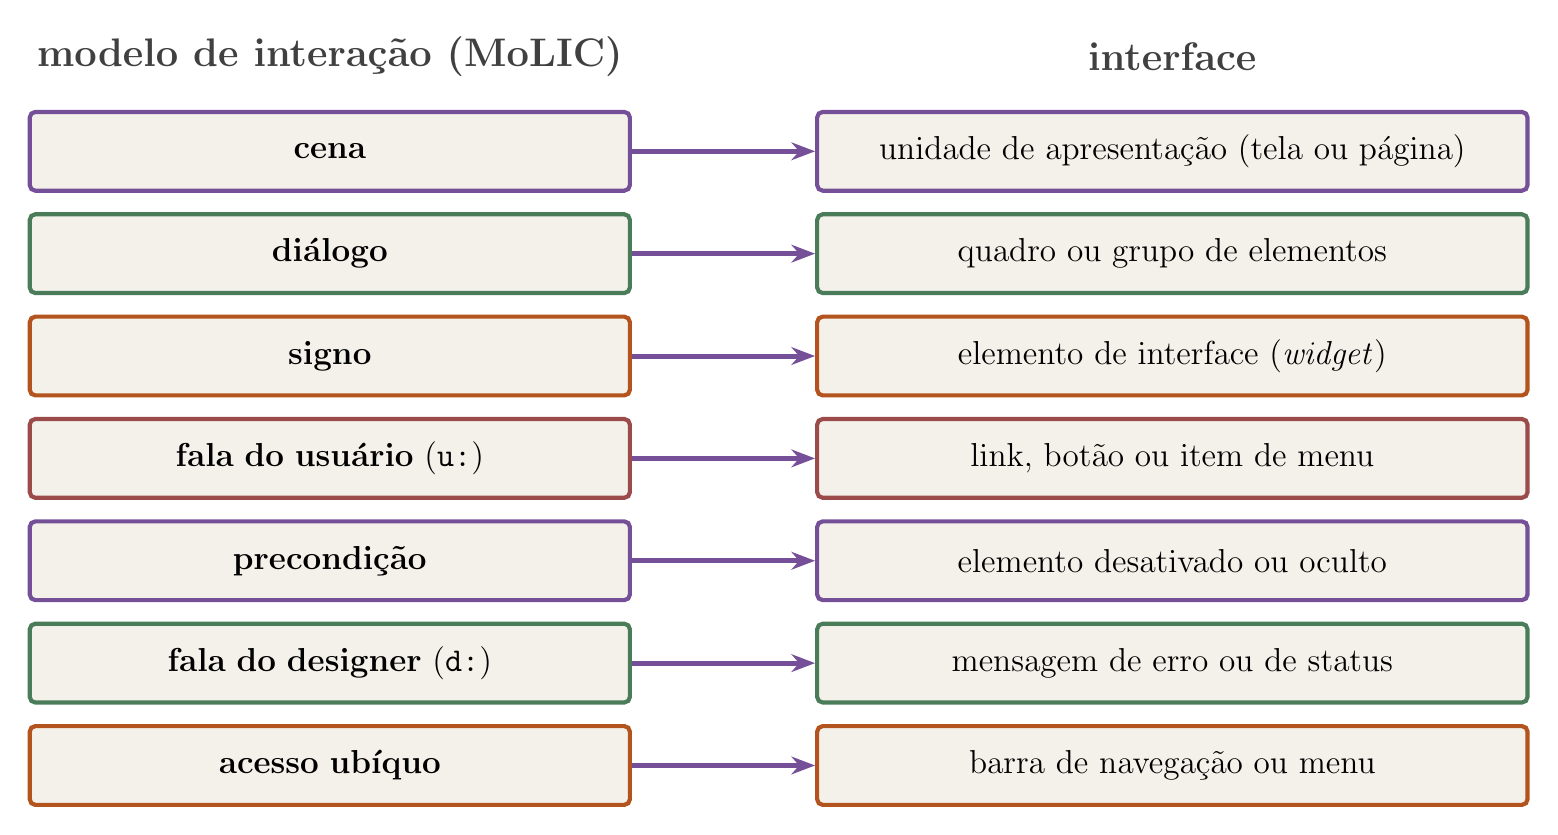
\begin{tikzpicture}[x=1cm,y=1cm]
\node[font=\Large\bfseries, black!75] at (3.9,8.6) {modelo de interação (MoLIC)};
\node[font=\Large\bfseries, black!75] at (14.6,8.6) {interface};
\node[dbox, draw=dblue, line width=1.5pt, text width=7.2cm, minimum height=1.0cm, font=\large] (l0) at (3.9,7.4) {\textbf{cena}};
\node[dbox, draw=dblue, line width=1.5pt, text width=8.6cm, minimum height=1.0cm, font=\large] (r0) at (14.6,7.4) {unidade de apresentação (tela ou página)};
\draw[dtrans, line width=1.8pt, -{Stealth[length=3mm]}] (l0.east) -- (r0.west);
\node[dbox, draw=dgreen, line width=1.5pt, text width=7.2cm, minimum height=1.0cm, font=\large] (l1) at (3.9,6.1) {\textbf{diálogo}};
\node[dbox, draw=dgreen, line width=1.5pt, text width=8.6cm, minimum height=1.0cm, font=\large] (r1) at (14.6,6.1) {quadro ou grupo de elementos};
\draw[dtrans, line width=1.8pt, -{Stealth[length=3mm]}] (l1.east) -- (r1.west);
\node[dbox, draw=dorange, line width=1.5pt, text width=7.2cm, minimum height=1.0cm, font=\large] (l2) at (3.9,4.8) {\textbf{signo}};
\node[dbox, draw=dorange, line width=1.5pt, text width=8.6cm, minimum height=1.0cm, font=\large] (r2) at (14.6,4.8) {elemento de interface (\emph{widget})};
\draw[dtrans, line width=1.8pt, -{Stealth[length=3mm]}] (l2.east) -- (r2.west);
\node[dbox, draw=dred, line width=1.5pt, text width=7.2cm, minimum height=1.0cm, font=\large] (l3) at (3.9,3.5) {\textbf{fala do usuário} (\texttt{u:})};
\node[dbox, draw=dred, line width=1.5pt, text width=8.6cm, minimum height=1.0cm, font=\large] (r3) at (14.6,3.5) {link, botão ou item de menu};
\draw[dtrans, line width=1.8pt, -{Stealth[length=3mm]}] (l3.east) -- (r3.west);
\node[dbox, draw=dblue, line width=1.5pt, text width=7.2cm, minimum height=1.0cm, font=\large] (l4) at (3.9,2.2) {\textbf{precondição}};
\node[dbox, draw=dblue, line width=1.5pt, text width=8.6cm, minimum height=1.0cm, font=\large] (r4) at (14.6,2.2) {elemento desativado ou oculto};
\draw[dtrans, line width=1.8pt, -{Stealth[length=3mm]}] (l4.east) -- (r4.west);
\node[dbox, draw=dgreen, line width=1.5pt, text width=7.2cm, minimum height=1.0cm, font=\large] (l5) at (3.9,0.9) {\textbf{fala do designer} (\texttt{d:})};
\node[dbox, draw=dgreen, line width=1.5pt, text width=8.6cm, minimum height=1.0cm, font=\large] (r5) at (14.6,0.9) {mensagem de erro ou de status};
\draw[dtrans, line width=1.8pt, -{Stealth[length=3mm]}] (l5.east) -- (r5.west);
\node[dbox, draw=dorange, line width=1.5pt, text width=7.2cm, minimum height=1.0cm, font=\large] (l6) at (3.9,-0.4) {\textbf{acesso ubíquo}};
\node[dbox, draw=dorange, line width=1.5pt, text width=8.6cm, minimum height=1.0cm, font=\large] (r6) at (14.6,-0.4) {barra de navegação ou menu};
\draw[dtrans, line width=1.8pt, -{Stealth[length=3mm]}] (l6.east) -- (r6.west);
\end{tikzpicture}
\end{document}
